\documentclass[11pt,letterpaper,titlepage]{article}

\usepackage{geometry}
\geometry{left=2cm,right=2cm,top=2cm,bottom=3cm}

\usepackage{setspace}
\onehalfspacing

\usepackage{multicol}
\setlength{\columnsep}{3em}

\usepackage{booktabs}

\usepackage[table,x11names]{xcolor}

\usepackage{multirow}

\usepackage{pgfgantt}

\usepackage{listings}

\usepackage{xcolor}
\definecolor{vgreen}{RGB}{104,180,104}
\definecolor{vblue}{RGB}{49,49,255}
\definecolor{vorange}{RGB}{255,143,102}

\lstdefinestyle{C-style}
{
    language=C,
    basicstyle=\small\ttfamily,
    keywordstyle=\color{vblue},
    identifierstyle=\color{black},
    commentstyle=\color{vgreen},
    % numbers=left,
    numberstyle=\tiny\color{black},
    numbersep=11pt,
    tabsize=4,
    moredelim=*[s][\colorIndex]{[}{]},
    literate=*{:}{:}1
}

\lstdefinestyle{txt-style}
{
    basicstyle=\small\ttfamily,
    % numbers=left,
    numbersep=11pt,
    tabsize=4,
    moredelim=*[s][\colorIndex]{[}{]},
    literate=*{:}{:}1
}

\usepackage{tikz}
\usetikzlibrary{shapes.geometric, arrows, positioning, fit,calc}
\newcommand*\circled[1]{\tikz[baseline=(char.base)]{
            \node[shape=circle,draw,inner sep=1pt] (char) {#1};}}
            
\usepackage{hyperref}
\hypersetup{
    colorlinks,
    citecolor=black,
    filecolor=black,
    linkcolor=black,
    urlcolor=black
}

\usepackage{pifont}

\usepackage[toc,page]{appendix}

\pagestyle{empty}
\usepackage{tikz}
\usetikzlibrary{shapes.geometric, arrows}

\usetikzlibrary{mindmap,trees}
\usepackage{verbatim}

\usepackage{indentfirst}
\setlength{\parindent}{2em}

\usepackage{listings}

\usepackage{chngcntr}
\counterwithin{section}{part}
\renewcommand\thesection{\arabic{section}}

\usepackage{graphicx}

\usepackage{subcaption}

\usepackage{fancyhdr}

\pagestyle{fancy}
\lhead{}
\rhead{}
\lfoot{ECEN 749 Section 601 Lab 3}
\cfoot{\thepage}
\rfoot{@Lei Wang (Wilson)}
\renewcommand{\headrulewidth}{0pt}
\renewcommand{\headwidth}{\textwidth}
\renewcommand{\footrulewidth}{0.4pt}
\newcommand{\RomanNumeralCaps}[1]
    {\MakeUppercase{\romannumeral #1}}

\makeatletter
\newcommand*\@lbracket{[}
\newcommand*\@rbracket{]}
\newcommand*\@colon{:}
\newcommand*\colorIndex{%
    \edef\@temp{\the\lst@token}%
    \ifx\@temp\@lbracket \color{black}%
    \else\ifx\@temp\@rbracket \color{black}%
    \else\ifx\@temp\@colon \color{black}%
    \else \color{vorange}%
    \fi\fi\fi
}
\makeatother

\usepackage{trace}

\begin{document}

\begin{titlepage}
  \centering
	{\scshape\large Texas A\&M University \par}
	\vspace{1cm}
	{\scshape\Large Department of Electrical and Computer Engineering \par}
	\vspace{4cm}
    \vspace{0.5cm}
	{\huge\bfseries ECEN 749 Microprocessor System Design\par}
	\vspace{4cm}
	{\Large Lab 2 Report (Section 601)\par}
	\vspace{1cm}
	{\Large Student: Lei Wang (Wilson)\par}
	\vspace{1cm}
	{\Large UIN: 829009485\par}
	\vspace{1cm}
	{\Large Instructor: Dr. Paul V. Gratz\par}
	\vspace{4cm}
	\vfill

  % Bottom of the page
	{\large Submitted: February 11th, 2020 \par}

\end{titlepage}

\newpage

\tableofcontents{}

\newpage

\part{Introduction}

The lab session aims at teaching students build their own IP, integrate the IP into the system and use C to use the IP. The lab focuses on a simple hardware multiplier implementation and no longer uses the soft processor introduced in the previous lab.

\part{Procedure}

\begin{enumerate}
    \item Create a Vivado project in a new folder. When selecting the hardware, choose \textbf{Boards} $\rightarrow$ \textbf{Zybo Z7-10}.
    
    \item Create a block design schematic with the \textbf{ZYNQ7 Processing System} IP added. Name the block design \textbf{Multiply}.
    
    \item Configure the \textbf{ZYNQ7 Processing System} IP by double clicking on it. Download the \textbf{.tcl} file provided for the lab session to the Vivado project directory. Click on \textbf{Presets} $\rightarrow$ \textbf{Apply Configuration} in the \textbf{Re-customize IP} window. Select the downloaded \textbf{.tcl} file. Uncheck all peripheral I/O pins but \textbf{UART 1} in the \textbf{Peripheral I/O Pins} tab.
    
    \item Click on \textbf{Tools} $\rightarrow$ \textbf{Create and Package IP} to open the \textbf{Create and Package New IP} window. Click on \textbf{Next} $\rightarrow$ \textbf{Create a new AXI4 peripheral} $\rightarrow$ \textbf{Next}.
    
    \item Give the IP a name and a short description. Keep the version number unchanged. Click on \textbf{Next}.
    
    \item Configure \textbf{Interface} according to the following table:
    
    \begin{table}[ht]
    \centering
    \begin{tabular}{@{}llll@{}}
    \toprule
    \begin{tabular}[c]{@{}l@{}}Interface\\ type:\end{tabular} & \begin{tabular}[c]{@{}l@{}}Interface\\ mode:\end{tabular} & \begin{tabular}[c]{@{}l@{}}Data\\ width:\end{tabular} & \begin{tabular}[c]{@{}l@{}}Number of\\ registers:\end{tabular} \\ \midrule
    Lite                                                      & Slave                                                     & 32                                                    & 4                                                              \\ \bottomrule
    \end{tabular}
    \caption{New IP interface configuration}
    \end{table}
    
    Check \textbf{Edit IP} and click \textbf{Finish}.
    
    \item Open \textbf{multiply\_v1\_0\_S00\_AXI.v} in the \textbf{source} window under \textbf{multiply\_v1\_0}. Comment out code that modifies value in \textbf{slv\_reg2}.
    
    \item Find the line \textbf{//Add user logic here}. Add the following code:
    
    \lstinputlisting[style={txt-style}]{added_Verilog.txt}
    
    \item Click on \textbf{Review and Package} $\rightarrow$ \textbf{Re-package} in the \textbf{Package IP} tab. Close the customized-IP project when done.
    
    \item Go back to the Vivado project that contains the ZYNQ processing system and Add the multiplier IP that is created. Run connection automation. Remember to select \textbf{All Automation}.
    
    \item Regenerate layout. The finished layout should look like the following:
    
    \begin{figure}[ht]
    \centering
    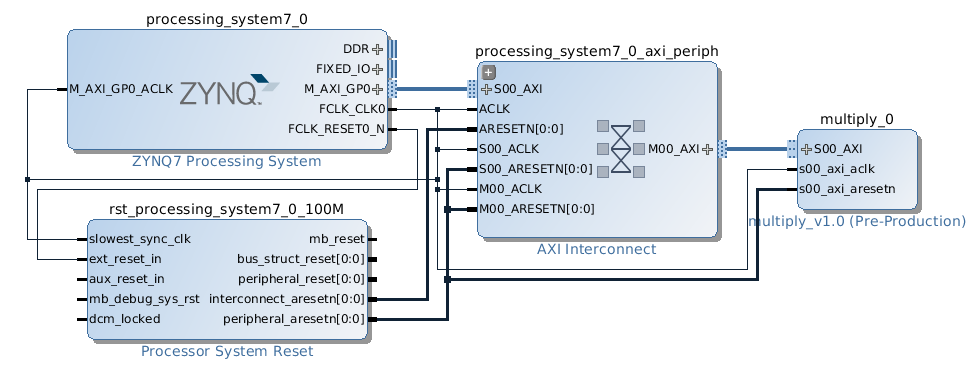
\includegraphics[width=\textwidth]{layout.png}
    \caption{Block design for lab 3.}
    \end{figure}
    
    \item Create HDL wrapper for the block design in the source tab.
    
    \item Generate the bitstream. Export the design, including the bitstream.
    
    \item Launch the Xilinx SDK. Create a \textbf{Hello World!} type \textbf{Application Project}.
    
    \item Open \textbf{helloworld.c}. Replace the code with the one in Appendix \ref{appendix:multiplier_c}.
    
    \item Program FPGA.
    
    \item Launch a terminal and run the following command:
    
    \verb|source /opt/coe/Xilinx/Vivado/2015.2/settings64.sh|
    
    \verb|picocom -b 115200 /dev/ttyUSB1|
    
    \item Run the program from the Xilinx SDK.
    
    \item The output is observed from the picocom console.
    
\end{enumerate}

\newpage

\part{Results}

The program takes one value from each of the two int arrays consecutively and use the multiplier IP to get the multiplication result of the two numbers. The result is list as the following. Note the result and the numbers are displayed in hexadecimal format.

\begin{figure}[ht]
    \centering
    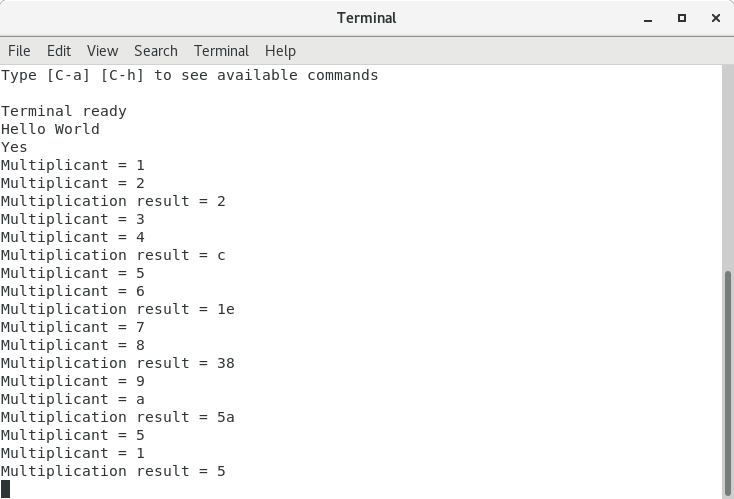
\includegraphics[width=\textwidth]{picocom.png}
    \caption{Picocom output.}
    \end{figure}

The multiplier handles multiplication successfully.

\newpage

\part{Conclusion}

In this lab, I have learnt to create a custom IP using Vivado and modify the logic in the Verilog code that is automatically generated by Vivado. Also, the use of the Arm processor and ways to communicate with the board is different from previous labs. The C program and where to look for parameters such as register addresses and functions such as write and read from registers remain the same: it is always going to be in \textbf{xparameters.h} and \textbf{xgpio.h}.

\textbf{Q: What is the purpose of the tmp\_reg from the Verilog code provided in lab, and what happens if
this register is removed from the code?}

A: tmp\_reg is used to temporarily hold the result of multiplication. After the result of multiplication has been generated, the result stays in tmp\_reg  and is transfered to slv\_reg2 for output. If tmp\_reg is removed, unpredictable behaviour may occur and the output may be random numbers. It is because the signals need time to propagate and the gates also propagation delays. It is impossible for signals to take no time to travel through all the wiring and gates in real life, though it is possible to do so in simulation. Hence a reg is needed to wait for the signals to arrive, hold the value and output in the next cycle.

\textbf{Q: What values of ‘slv\_reg0’ and ‘slv\_reg1’ would produce incorrect results from the multiplication
block? What is the name commonly assigned to this type of computation error, and how would
you correct this? Provide a Verilog example and explain what you would change during the
creation of the corrected peripheral.}

A: Any pairs of values that yield a multiplication result that is greater than $2^{31}-1$. This type of computation error is known as overflow. To correct this, recall our IP has 4 registers while one of them is not used. Hence we can store the high-32 bit of our multiplication result in the 4th register and store the low-32 bit of the multiplication result in the 3rd register, assuming our multiplication result is put into a 64-bit format instead of the 32-bit form used in this lab session. The modified Verilog code will be the following:

\lstinputlisting[style={txt-style}]{64-bit_Verilog.txt}

The code that writes to slv\_reg3 needs to be commented out and to use the multiplier, additional read operations are needed in the C program in order to retrieve the complete 64-bit multiplication result.

% if have time, test the 64-bit multiplier with modified C code

\newpage

\begin{appendices}

\section{Multiplier.c}
\label{appendix:multiplier_c}
\lstinputlisting[style={C-style}]{lab3.c}

\end{appendices}

\end{document}
